\documentclass[12pt]{article}
\usepackage{graphicx}
\usepackage[margin=2cm]{geometry}
\usepackage[utf8]{inputenc}
\usepackage{tikz}
\usepackage[export]{adjustbox}
\usepackage{indentfirst}
\usepackage{wrapfig}
\usepackage{listings}
\usepackage{color}
\usepackage{enumerate}
\usepackage{amssymb, bm}
\usepackage{amsmath}
\usepackage{csvsimple}
\usepackage{tikz}
\usetikzlibrary{positioning}
\usepackage{lscape}
\newcommand\tab[1][1cm]{\hspace*{#1}}
\definecolor{mygreen}{rgb}{0,0.6,0}
\definecolor{mygray}{rgb}{0.5,0.5,0.5}
\definecolor{mymauve}{rgb}{0.58,0,0.82}
\lstset{ %
    backgroundcolor=\color{gray!10!white},
  basicstyle=\tiny, %footnotesize,        % the size of the fonts that are used for the code
  breakatwhitespace=false,         % sets if automatic breaks should only happen at whitespace
  breaklines=true,                 % sets automatic line breaking
  captionpos=b,                    % sets the caption-position to bottom
  commentstyle=\color{mygreen},    % comment style
  deletekeywords={...},            % if you want to delete keywords from the given language
  escapeinside={\%*}{*)},          % if you want to add LaTeX within your code
  extendedchars=true,              % lets you use non-ASCII characters; for 8-bits encodings only, does not work with UTF-8
  frame=single,	                   % adds a frame around the code
  keepspaces=true,                 % keeps spaces in text, useful for keeping indentation of code (possibly needs columns=flexible)
  keywordstyle=\color{blue},       % keyword style
  language=Python,                 % the language of the code
  morekeywords={*,...},           % if you want to add more keywords to the set
  numbers=left,                    % where to put the line-numbers; possible values are (none, left, right)
  numbersep=10pt,                   % how far the line-numbers are from the code
  numberstyle=\tiny\color{mygray}, % the style that is used for the line-numbers
  rulecolor=\color{black},         % if not set, the frame-color may be changed on line-breaks within not-black text (e.g. comments (green here))
  showspaces=false,                % show spaces everywhere adding particular underscores; it overrides 'showstringspaces'
  showstringspaces=false,          % underline spaces within strings only
  showtabs=false,                  % show tabs within strings adding particular underscores
  stepnumber=1,                    % the step between two line-numbers. If it's 1, each line will be numbered
  stringstyle=\color{mymauve},     % string literal style
  tabsize=1,	                   % sets default tabsize to 2 spaces
  title=\lstname                   % show the filename of files included with \lstinputlisting; also try caption instead of title
}
\graphicspath{ }
\usetikzlibrary{arrows}

\title{\textbf{COMP0085 Summative Assignment}}
%\author{Jian Shu (James) Wu \\ }
\date{Jan 4, 2023}

\begin{document}
\maketitle
\section*{Question 1}

\subsection*{(a)} The directed acyclic graph:

\begin{center}
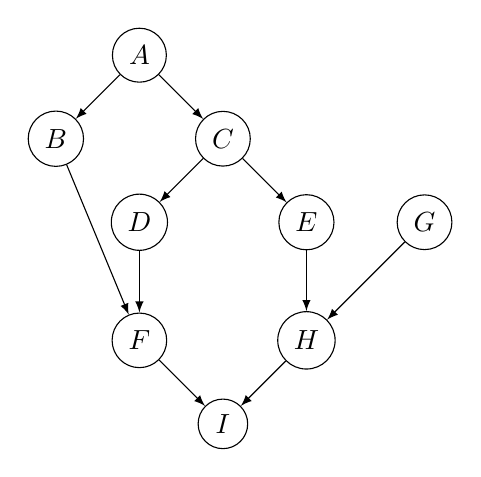
\begin{tikzpicture}[node distance={15mm}, main/.style = {draw, circle}]
    \node[main] (A) {$A$};
    \node[main] (B) [below left of=A] {$B$};
    \node[main] (C) [below right of=A] {$C$};
    \node[main] (E) [below right of=C] {$E$};
    \node[main] (D) [below left of=C] {$D$};
    \node[main] (H) [below of=E] {$H$};
    \node[main] (G) [right of=E] {$G$};
    \node[main] (I) [below left of=H] {$I$};
    \node[main] (F) [above left of=I] {$F$};

    \draw[-latex] (A) -- (B);
    \draw[-latex] (A) -- (C);
    \draw[-latex] (B) -- (F);
    \draw[-latex] (C) -- (D);
    \draw[-latex] (C) -- (E);
    \draw[-latex] (G) -- (H);
    \draw[-latex] (D) -- (F);
    \draw[-latex] (E) -- (H);
    \draw[-latex] (F) -- (I);
    \draw[-latex] (H) -- (I);
\end{tikzpicture}
\end{center}


\subsection*{(b)} The moralised graph:

\begin{center}
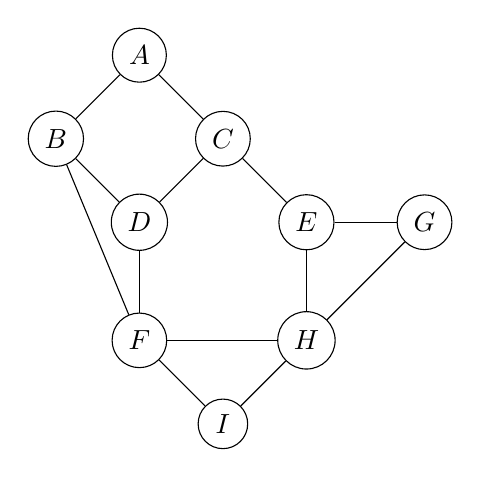
\begin{tikzpicture}[node distance={15mm}, main/.style = {draw, circle}]
    \node[main] (A) {$A$};
    \node[main] (B) [below left of=A] {$B$};
    \node[main] (C) [below right of=A] {$C$};
    \node[main] (E) [below right of=C] {$E$};
    \node[main] (D) [below left of=C] {$D$};
    \node[main] (H) [below of=E] {$H$};
    \node[main] (G) [right of=E] {$G$};
    \node[main] (I) [below left of=H] {$I$};
    \node[main] (F) [above left of=I] {$F$};

    \draw (A) -- (B);
    \draw (A) -- (C);
    \draw (B) -- (F);
    \draw (B) -- (D);
    \draw (C) -- (D);
    \draw (C) -- (E);
    \draw (E) -- (G);
    \draw (G) -- (H);
    \draw (D) -- (F);
    \draw (E) -- (H);
    \draw (F) -- (H);
    \draw (F) -- (I);
    \draw (H) -- (I);
\end{tikzpicture}
\end{center}

\newpage

An effective triangulation:

%\begin{center}
%\begin{tikzpicture}[node distance={15mm}, main/.style = {draw, circle}]
%    \node[main] (A) {$A$};
%    \node[main] (B) [below left of=A] {$B$};
%    \node[main] (C) [below right of=A] {$C$};
%    \node[main] (E) [below right of=C] {$E$};
%    \node[main] (D) [below left of=C] {$D$};
%    \node[main] (H) [below of=E] {$H$};
%    \node[main] (G) [right of=E] {$G$};
%    \node[main] (I) [below left of=H] {$I$};
%    \node[main] (F) [above left of=I] {$F$};
%
%    \draw (A) -- (B);
%    \draw (A) -- (C);
%    \draw (B) -- (F);
%    \draw (B) -- (D);
%    \draw (C) -- (D);
%    \draw (C) -- (E);
%    \draw (E) -- (G);
%    \draw (G) -- (H);
%    \draw (D) -- (F);
%    \draw (E) -- (H);
%    \draw (F) -- (H);
%    \draw (F) -- (I);
%    \draw (H) -- (I);
%
%    \draw[dashed] (I) -- (E);
%    \draw[dashed] (F) -- (E);
%    \draw[dashed] (C) -- (F);
%    \draw[dashed] (B) -- (D);
%    \draw[dashed] (B) -- (C);
%
%\end{tikzpicture}
%\end{center}


\begin{center}
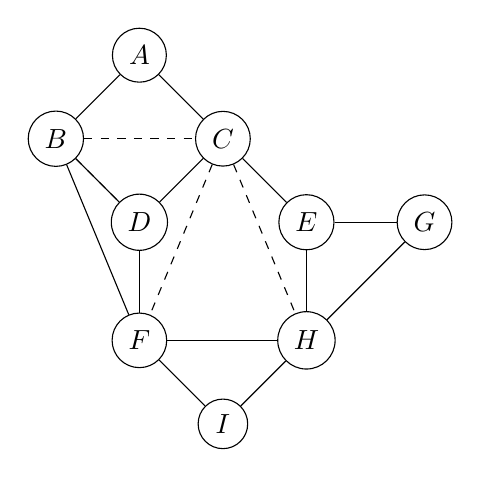
\begin{tikzpicture}[node distance={15mm}, main/.style = {draw, circle}]
    \node[main] (A) {$A$};
    \node[main] (B) [below left of=A] {$B$};
    \node[main] (C) [below right of=A] {$C$};
    \node[main] (E) [below right of=C] {$E$};
    \node[main] (D) [below left of=C] {$D$};
    \node[main] (H) [below of=E] {$H$};
    \node[main] (G) [right of=E] {$G$};
    \node[main] (I) [below left of=H] {$I$};
    \node[main] (F) [above left of=I] {$F$};

    \draw (A) -- (B);
    \draw (A) -- (C);
    \draw (B) -- (F);
    \draw (B) -- (D);
    \draw (C) -- (D);
    \draw (C) -- (E);
    \draw (E) -- (G);
    \draw (G) -- (H);
    \draw (D) -- (F);
    \draw (E) -- (H);
    \draw (F) -- (H);
    \draw (F) -- (I);
    \draw (H) -- (I);

    \draw[dashed] (C) -- (H);
    \draw[dashed] (C) -- (F);
    \draw[dashed] (B) -- (D);
    \draw[dashed] (B) -- (C);

\end{tikzpicture}
\end{center}

where the dashed lines are edges added to triangulate the moralised graph.

\newpage

The resulting junction tree:



%\begin{center}
%\begin{tikzpicture}[node distance={15mm}, main/.style = {draw, circle}, square/.style={regular polygon,regular polygon sides=4}]
%    \node[main] (ABC) {$ABC$};
%    \node[square] (BC) [square,draw] [below of=ABC] {$BC$};
%    \node[main] (BCDF) [below of=BC] {$BCDF$};
%    \node[square] (CF) [square,draw] [below of=BCDF] {$CF$};
%    \node[main] (CEF) [below of=CF] {$CEF$};
%    \node[square] (EF) [square,draw] [below of=CEF] {$EF$};
%    \node[main] (EFHI) [below of=EF] {$EFHI$};
%    \node[square] (EH) [square,draw] [below of=EFHI] {$EH$};
%    \node[main] (EGH) [below of=EH] {$EGH$};
%    \draw (ABC) -- (BC);
%    \draw (BC) -- (BCDF);
%    \draw (BCDF) -- (CF);
%    \draw (CF) -- (CEF);
%    \draw (CEF) -- (EF);
%    \draw (EF) -- (EFHI);
%    \draw (EFHI) -- (EH);
%    \draw (EH) -- (EGH);
%\end{tikzpicture}
%\end{center}

\begin{center}
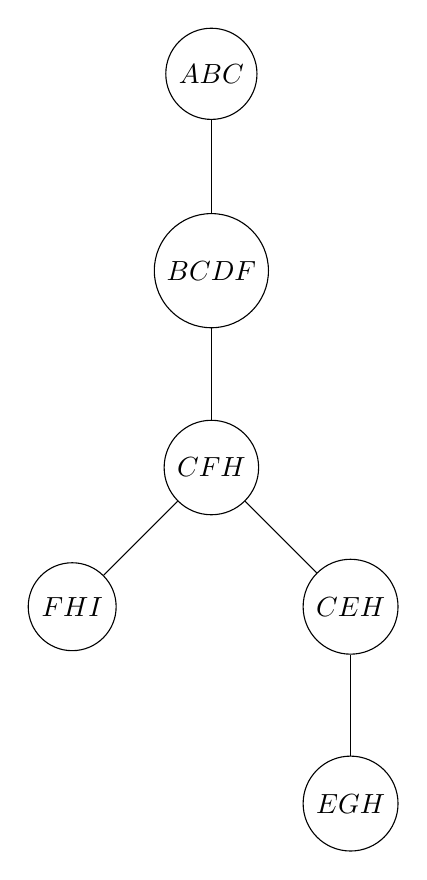
\begin{tikzpicture}[node distance={25mm}, main/.style = {draw, circle}, square/.style={regular polygon,regular polygon sides=4}]
    \node[main] (ABC) {$ABC$};
    \node[main] (BCDF) [below of=ABC] {$BCDF$};
    \node[main] (CFH) [below of=BCDF] {$CFH$};
    \node[main] (FHI) [below left of=CFH] {$FHI$};
    \node[main] (CEH) [below right of=CFH] {$CEH$};
    \node[main] (EGH) [below of=CEH] {$EGH$};
    \draw (ABC) -- (BCDF);
    \draw (BCDF) -- (CFH);
    \draw (CFH) -- (FHI);
    \draw (CFH)  -- (CEH);
    \draw (EGH)  -- (CEH);
\end{tikzpicture}
\end{center}

where the circular nodes are cliques.

\newpage

The junction tree redrawn as a factor graph:

\begin{center}
\begin{tikzpicture}[node distance={15mm}, main/.style = {draw, circle}, square/.style={regular polygon,regular polygon sides=4}]
    \node[main] (ABC) {$ABC$};
    \node[square] (BC) [square,draw] [below of=ABC] {$BC$};
    \node[main] (BCDF) [below of=BC] {$BCDF$};
    \node[square] (CF) [square,draw] [below of=BCDF] {$CF$};
    \node[main] (CFH) [below of=CF] {$CFH$};
    \node[square] (FH) [square,draw] [below left of=CFH] {$FH$};
    \node[main] (FHI) [below left of=FH] {$FHI$};
    \node[square] (CH) [square,draw] [below right of=CFH] {$CH$};
    \node[main] (CEH) [below right of=CH] {$CEH$};
    \node[square] (EH) [square,draw] [below of=CEH] {$EH$};
    \node[main] (EGH) [below of=EH] {$EGH$};
    \draw (ABC) -- (BC);
    \draw (BC) -- (BCDF);
    \draw (BCDF) -- (CF);
    \draw (CF) -- (CFH);
    \draw (CFH) -- (FH);
    \draw (FH) -- (FHI);
    \draw (CFH) -- (CH);
    \draw (CH) -- (CEH);
    \draw (CEH) -- (EH);
    \draw (EGH) -- (EH);
\end{tikzpicture}
\end{center}

where the circular nodes are cliques and the square nodes are separators/factors.

\newpage

\subsection*{(c)}

\begin{center}
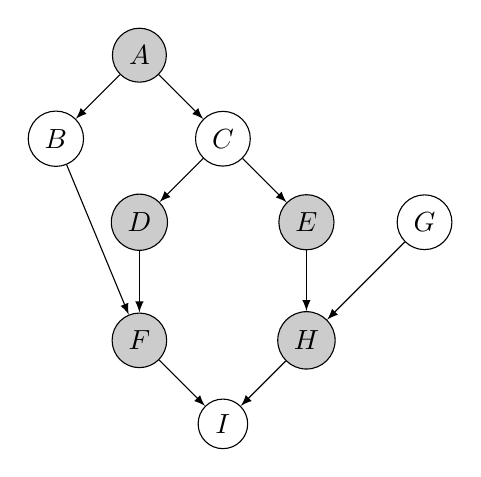
\begin{tikzpicture}[node distance={15mm}, main/.style = {draw, circle}]
    \node[main] (A) [fill=black!20] {$A$};
    \node[main] (B) [below left of=A] {$B$};
    \node[main] (C) [below right of=A] {$C$};
    \node[main] (E) [below right of=C, fill=black!20] {$E$};
    \node[main] (D) [below left of=C, fill=black!20] {$D$};
    \node[main] (H) [below of=E, fill=black!20] {$H$};
    \node[main] (G) [right of=E] {$G$};
    \node[main] (I) [below left of=H] {$I$};
    \node[main] (F) [above left of=I, fill=black!20] {$F$};

    \draw[-latex] (A) -- (B);
    \draw[-latex] (A) -- (C);
    \draw[-latex] (B) -- (F);
    \draw[-latex] (C) -- (D);
    \draw[-latex] (C) -- (E);
    \draw[-latex] (G) -- (H);
    \draw[-latex] (D) -- (F);
    \draw[-latex] (E) -- (H);
    \draw[-latex] (F) -- (I);
    \draw[-latex] (H) -- (I);
\end{tikzpicture}
\end{center}


The set $\{A, D, E, F, H\}$ is a non-unique smallest set of molecules such that if the concentrations of the species within the set are known, the concentrations of the others $\{B, C, G, I\}$ would all be independent (conditioned on the measured ones).


\subsection*{(d)}

\newpage

\subsection*{(e)}

\newpage
\section*{Question 2}

\subsection*{(a)}

We want the posterior mean and covariance over $a$ and $b$.
Defining a weight vector $\textbf{w}$:

\[\textbf{w} = \begin{bmatrix}
                 a \\
                 b
         \end{bmatrix}\]

Our distribution for $\textbf{w}$:

\[P(\textbf{w}) = \mathcal{N} \left(
\begin{bmatrix}
                 \mu_a \\
                 \mu_b
         \end{bmatrix} ,
\begin{bmatrix}
                 \sigma_a^2 & 0 \\
                 0 & \sigma_b^2
         \end{bmatrix}
\right)
  = \mathcal{N}(\mu_{\textbf{w}}, \Sigma_{\textbf{w}})
\]

Moreover, for our data $\mathcal{D} = \{\textbf{X}, \textbf{Y}\}$:

\[P(\mathcal{D} | \textbf{w}) = \mathcal{N} \left( \textbf{Y} - \textbf{w}^T \textbf{X}, \sigma^2 \textbf{I}
\right)
\]

where $\textbf{X} =  \begin{bmatrix}
                 t_1 & t_2 \cdots t_N \\
                 1 & 1 \cdots 1
         \end{bmatrix} \in  \mathbb{R}^{2 \times N}$ and $\textbf{Y} \in \mathbb{R}^{1 \times N}$.

Knowing:

\[P(\textbf{w} | \mathcal{D}) \propto P(\mathcal{D} | \textbf{w}) P(\textbf{w})\]

we can substitute the above distributions:

\[P(\textbf{w} | \mathcal{D}) \propto
  \exp \left(\frac{-1}{2 \sigma^2} \left( \textbf{Y} - \textbf{w}^T \textbf{X}\right) \left( \textbf{Y} - \textbf{w}^T \textbf{X}\right)^T \right)
\exp \left(\frac{-1}{2} \left( \textbf{w} -\mu_{\textbf{w}}\right)^T \Sigma_{\textbf{w}}^{-1} \left( \textbf{w} -\mu_{\textbf{w}}\right)\right)
\]

expanding:

\[\log P(\textbf{w} | \mathcal{D}) \propto
  \frac{-1}{2} \left( \frac{\textbf{Y} \textbf{Y}^T}{\sigma^2} - 2\textbf{w}^T \frac{\textbf{X}\textbf{Y}^T}{\sigma^2} + \textbf{w}^T \frac{\textbf{X} \textbf{X}^T}{\sigma^2} \textbf{w} +  \textbf{w}^T \Sigma_{\textbf{w}}^{-1}  \textbf{w} - 2\textbf{w}^T \Sigma_{\textbf{w}}^{-1}\mu_{\textbf{w}} + \mu_{\textbf{w}}^T\Sigma_{\textbf{w}}^{-1}\mu_{\textbf{w}} \right)
\]

collecting $\textbf{w}$ terms:

\[\log P(\textbf{w} | \mathcal{D}) \propto
  \frac{-1}{2} \left( \textbf{w}^T \left(\frac{\textbf{X} \textbf{X}^T}{\sigma^2} + \Sigma_{\textbf{w}}^{-1} \right)  \textbf{w} - 2\textbf{w}^T \left(\frac{\textbf{X}\textbf{Y}^T}{\sigma^2} + \Sigma_{\textbf{w}}^{-1} \mu_{\textbf{w}}\right)  \right)
\]

Knowing that the posterior $P(\textbf{w} | \mathcal{D})$ will be Gaussian with mean $\bar{\mu}_w$ and covariance $\bar{\Sigma}_w$, we can see that expanding the exponent component would have the form:

\[\left( \textbf{w} - \bar{\mu}_w \right)^T \bar{\Sigma}_w^{-1} \left( \textbf{w} - \bar{\mu}_w \right) = \textbf{w}^T \bar{\Sigma}_w^{-1} \textbf{w} -2 \textbf{w}^T \bar{\Sigma}_w^{-1} \bar{\mu}_w + \bar{\mu}_w^T \bar{\Sigma}_w^{-1} \bar{\mu}_w\]

Thus we can identify the posterior covariance:

\[\bar{\Sigma}_w = \left(\frac{\textbf{X} \textbf{X}^T}{\sigma^2} + \Sigma_{\textbf{w}}^{-1} \right)^{-1}\]


and the posterior mean:

\[\bar{\mu}_w = \bar{\Sigma}_w \left(\frac{\textbf{X}\textbf{Y}^T}{\sigma^2} + \Sigma_{\textbf{w}}^{-1} \mu_{\textbf{w}}\right) \]

\newpage
The Python code:
\lstinputlisting[language=Python]{src/solutions/q2.py}

\newpage
\section*{Question 3}

\subsection*{(a)}

The free energy is can be calculated as:
\[\mathcal{F}(q, \theta) = \langle \log P(\textbf{x}, \textbf{s} | \theta)\rangle_{q(\textbf{s})} + H[Q(\textbf{s})]\]


%Thus,
%\[\mathcal{F}(Q, \theta) = \langle \log P(\textbf{x}, \textbf{s} | \theta)\rangle_{\prod_{i=1}^{K} q_{i} (s_i)} + H\left[ \prod_{i=1}^{K} q_{i} (s_i)\right] \]

Knowing,
\[\log P(\textbf{x}, \textbf{s} | \theta) = \log P(\textbf{x} | \textbf{s}, \theta) + \log P(\textbf{s} | \theta)\]

we can write:

\[\mathcal{F}(Q, \theta) = \langle \log P(\textbf{x} | \textbf{s}, \theta)\rangle_{q(\textbf{s})} + \langle \log P(\textbf{s} | \theta)\rangle_{q(\textbf{s})} + H\left[ q(\textbf{s})\right] \]

Moreover, our mean field approximation:
\[q(\textbf{s}) = \prod_{i=1}^{K} q_{i} (s_i) \]

where $q_{i} (s_i) = \lambda_i^{s_i} (1-\lambda_i)^{(1-s_i)}$.


To compute the first term:

\[ P(\textbf{x} | \textbf{s}, \theta)  = \mathcal{N}\left( \sum_{i=1}^{K} s_i \mu_i, \sigma^2 \textbf{I} \right)}\]

substituting the appropriate terms:

\[ P(\textbf{x} | \textbf{s}, \theta)  = 2\pi^{-\frac{d}{2}} |\sigma^2 \textbf{I}|^{-\frac{1}{2}} \exp \left( -\frac{1}{2} \left(\textbf{x} - \sum_{i=1}^{K} s_i \mu_i\right)^T \frac{1}{\sigma^2} \textbf{I}  \left(\textbf{x} - \sum_{i=1}^{K} s_i \mu_i\right) \right) \]

with $d$ being the number of dimensions.


Taking the logarithm:

\[ \log P(\textbf{x} | \textbf{s}, \theta)  = -\frac{d}{2} \log (2 \pi \sigma^2)  -\frac{1}{2 \sigma^2} \left(\textbf{x}^T\textbf{x} - 2 \textbf{x}^T\sum_{i=1}^{K} s_i \mu_i   + \sum_{i=1}^{K} \sum_{i=1}^{K} s_i s_j \mu_i^T\mu_j \right) \]

The expectation distributed to the relevant terms:

\[
\langle \log P(\textbf{x} | \textbf{s}, \theta)\rangle_{q(\textbf{s})} \\
= -\frac{d}{2} \log (2 \pi \sigma^2)   -\frac{1}{2 \sigma^2} \left(\textbf{x}^T\textbf{x} - 2 \textbf{x}^T\sum_{i=1}^{K} \langle s_i \rangle_{q_{i} (s_i)} \mu_i   + \sum_{i=1}^{K} \sum_{j=1}^{K} \langle s_i s_j \rangle_{q_{i} (s_i) q_{j} (s_j)} \mu_i^T\mu_j \right)\]

Evaluating the expectations:

\[
\langle \log P(\textbf{x} | \textbf{s}, \theta)\rangle_{q(\textbf{s})} \\
= -\frac{d}{2} \log (2 \pi \sigma^2)  -\frac{1}{2 \sigma^2} \left(\textbf{x}^T\textbf{x} - 2 \textbf{x}^T\sum_{i=1}^{K}  \lambda_i  \mu_i   + \sum_{i=1}^{K} \sum_{j=1, j\neq i}^{K}  \lambda_i \lambda_j \mu_i^T\mu_j + \sum_{i=1}^{K}  \lambda_i \mu_i^T\mu_i \right)\]

where $\langle s_i s_i \rangle_{q_{i} (s_i)} = \langle s_i \rangle_{q_{i} (s_i)}$ because $s_i \in \{0, 1\}$.

To compute the second term:
\[ P(\textbf{s} | \theta) = \prod_{i=1}^{K}\pi_i^{s_i} (1-\pi_i)^{(1-s_i)}\]

Taking the logarithm:

\[ \log P(\textbf{s} | \theta) = \sum_{i=1}^{K}s_i \log \pi_i + (1-s_i) \log (1-\pi_i)}\]

The expectation distributed to the relevant terms:

\[ \langle \log P(\textbf{s} | \theta)\rangle_{q(\textbf{s})}= \sum_{i=1}^{K} \langle s_i \rangle_{q_{i} (s_i)} \log \pi_i + (1-\langle s_i\rangle_{q_{i} (s_i)}) \log (1-\pi_i)}\]

Evaluating the expectations:

\[ \langle \log P(\textbf{s} | \theta)\rangle_{q(\textbf{s})}= \sum_{i=1}^{K} \lambda_i \log \pi_i + (1-\lambda_i) \log (1-\pi_i)}\]

To compute the third term, we use the mean field factorisation:

\[H\left[ q(\textbf{s})\right] = \sum_{i=1}^K H\left[ q_{i} (s_i)\right] \]

Thus,

\[H\left[ q(\textbf{s})\right] = - \sum_{i=1}^K \sum_{s_i \in \{0, 1\}} q_{i} (s_i) \log q_{i} (s_i) \]

Substituting the appropriate values:

\[H\left[ q(\textbf{s})\right] = - \sum_{i=1}^K \lambda_i \log \lambda_i + (1-\lambda_i) \log (1-\lambda_i) \]

Combining, we have our free energy expression:


\[
\begin{array}{l}
\tab \mathcal{F}(q, \theta) = \\
\tab \tab \frac{-d}{2} \log (2 \pi \sigma^2)   -\frac{1}{2 \sigma^2} \left(\textbf{x}^T\textbf{x} - 2 \textbf{x}^T\sum_{i=1}^{K}  \lambda_i  \mu_i   + \sum_{i=1}^{K} \sum_{j=1, j\neq i}^{K}  \lambda_i \lambda_j \mu_i^T\mu_j + \sum_{i=1}^{K}  \lambda_i \mu_i^T\mu_i \right) \\
\tab \tab + \sum_{i=1}^{K} \lambda_i \log \pi_i + (1-\lambda_i) \log (1-\pi_i)}\\
\tab \tab - \sum_{i=1}^K \lambda_i \log \lambda_i + (1-\lambda_i) \log (1-\lambda_i)
\end{array}
\]

To derive the partial update for $q_i(s_i)$ we take the variational derivative of the Lagrangian, enforcing the normalisation of $q_i$:

\[\frac{\partial}{\partial q_i}\left( \mathcal{F}(q, \theta) + \lambda^{LG} \int q_i -1)\right) = \langle \log P(\textbf{x}, \textbf{s} | \theta)\rangle_{\prod_{j\neq i} q_j(s_j)} - \log q_i(s_i) - 1 + \lambda^{LG}\]

where $\lambda^{LG}$ is the Lagrange multiplier.

Setting this to zero we can solve for the $\lambda_i$ that maximises the free energy:

\[\log q_i(s_i) = \langle \log P(\textbf{x}, \textbf{s} | \theta)\rangle_{\prod_{j\neq i} q_j(s_j)} - 1 + \lambda^{LG}\]


Similar to our free energy derivation:

\[\langle \log P(\textbf{x} |  \textbf{s}, \theta)\rangle_{\prod_{j\neq i} q_j(s_j)} \propto  -\frac{1}{2 \sigma^2} \left(\textbf{x}^T\textbf{x} - 2 \textbf{x}^T\sum_{k=1}^{K} \langle s_k \rangle_{\prod_{j\neq i} q_j(s_j)} \mu_i   + \sum_{k=1}^{K} \sum_{j=1}^{K} \langle s_k s_j \rangle_{\prod_{j\neq i} q_j(s_j)} \right)\]

and

\[ \langle \log P(\textbf{s} | \theta)\rangle_{\prod_{j\neq i} q_j(s_j)} = \sum_{k=1}^{K} \langle s_k \rangle_{\prod_{j\neq i} q_j(s_j)} \log \pi_k + (1-\langle s_k\rangle_{\prod_{j\neq i} q_j(s_j)}) \log (1-\pi_k)}\]

We can write:

\[\log q_i(s_i) \propto  \log P(\textbf{x} |  \textbf{s}, \theta)\rangle_{\prod_{j\neq i} q_j(s_j)} + \langle \log P(\textbf{s} | \theta)\rangle_{\prod_{j\neq i} q_j(s_j)} \]

Substituting the relevant terms:

\[\log q_i(s_i) \propto  -\frac{1}{2 \sigma^2} \left( - 2 s_i \textbf{x}^T \mu_i   + s_i s_i  \mu_i^T\mu_i +  2 \sum_{j=1, j\neq i}^{K}  s_i \lambda_j  \mu_i^T\mu_j  \right) + s_i \log \pi_i + (1- s_i ) \log (1-\pi_i)}
\]

Knowing $\log q_i(s_i) = s_i \log \lambda_i + (1-s_i) \log (1-\lambda_i)$:

\[\log q_i(s_i) \propto s_i \log \frac{\lambda_i}{1-\lambda_i}\]

Thus,

\[s_i \log \frac{\lambda_i}{1-\lambda_i} \propto  -\frac{1}{2 \sigma^2} \left( - 2 s_i \textbf{x}^T \mu_i   + s_i s_i  \mu_i^T\mu_i +  2 \sum_{j=1, j\neq i}^{K}  s_i \lambda_j  \mu_i^T\mu_j  \right) + s_i \log \frac{\pi_i}{1-\pi_i}}\]

Also, because $s_i \in \{0, 1\}}$ we know that $s_i^2 = s_i$:

\[s_i \log \frac{\lambda_i}{1-\lambda_i} \propto  -\frac{1}{2 \sigma^2} \left( - 2 s_i \textbf{x}^T \mu_i   +  s_i  \mu_i^T\mu_i +  2 \sum_{j=1, j\neq i}^{K}  s_i \lambda_j  \mu_i^T\mu_j  \right) + s_i \log \frac{\pi_i}{1-\pi_i}}\]

Because we have only kept terms with $s_i$, this is an equality:

\[s_i \log \frac{\lambda_i}{1-\lambda_i} =  \frac{  s_i \mu_i^T}{2 \sigma^2} \left( 2\textbf{x} - \mu_i -  2 \sum_{j=1, j\neq i}^{K}   \lambda_j  \mu_j \right) + s_i \log \frac{\pi_i}{1-\pi_i}}\]

Solving for $\lambda_i$:

\[ \lambda_i =  \frac{1}{1+\exp\left[ - \left(\frac{  \mu_i^T}{\sigma^2} \left( \textbf{x} -  \frac{\mu_i}{2} -  \sum_{j=1, j\neq i}^{K}   \lambda_j  \mu_j \right) + \log \frac{\pi_i}{1-\pi_i}}\right) \right]}\]

we have our partial update.

\newpage
The Python code:
\lstinputlisting[language=Python]{src/solutions/q3.py}
\newpage
\section*{Question 4}

\newpage
\section*{Question 5}

\subsection*{(a)}

The log-joint probability for a single observation-source pair:

\[\log p(\textbf{s}, \textbf{x}) = \log p(\textbf{s}) + \logp(\textbf{x}|\textbf{s})\]

Knowing $p(\textbf{s}) = \prod_{i=1}^{K}p(s_i| \pi_i)$ and $p(\textbf{x}|\textbf{s}) = \mathcal{N}(\sum_{i=1}^{K} s_i \mu_i, \sigma^2 \textbf{I})$:

\[\log p(\textbf{s}, \textbf{x})  \propto \frac{-1}{2}\left( \textbf{x} - \sum_{i=1}^{K}s_i \mu_i\right)^T \frac{1}{\sigma^2} \textbf{I} \left( \textbf{x} - \sum_{i=1}^{K} s_i \mu_i\right) + \sum_{i=1}^{K} \left(s_i \log\pi_i + (1-s_i)\log(1-\pi_i)\right)\]

Expanding:

\[\log p(\textbf{s}, \textbf{x})  \propto \frac{-1}{2\sigma^2} \left( \textbf{x}^T\textbf{x} - 2\textbf{x}^T\sum_{i=1}^{K}s_i \mu_i + \sum_{i=1}^{K}\sum_{j=1}^{K}s_i s_j \mu_i^T \mu_j\right) + \sum_{i=1}^{K} \left(s_i \log\pi_i + (1-s_i)\log(1-\pi_i)\right)\]

Collecting terms pertaining to $s_i$:

\[\log p(\textbf{s}, \textbf{x})  =    \sum_{i=1}^{K} \left(\left(\frac{\textbf{x}^T \mu_i}{\sigma^2} +\log\frac{\pi_i}{1-\pi_i} \right) s_i\right) + \sum_{i=1}^{K}\sum_{j=1}^{K}\left( \frac{ - \mu_i^T \mu_j}{2\sigma^2} s_i s_j \right) + C\]

where $C$ are all other terms without $s_i$.

Knowing that $s_i^2= s_i$:

\[\log p(\textbf{s}, \textbf{x})  =    \sum_{i=1}^{K} \left(\left(\frac{\textbf{x}^T \mu_i}{\sigma^2} +\log\frac{\pi_i}{1-\pi_i} - \frac{\mu_i^T \mu_j}{2\sigma^2} \right) s_i\right) + \sum_{i=1}^{K}\sum_{j=1}^{i-1}\left( \frac{ - \mu_i^T \mu_j}{\sigma^2} s_i s_j \right) + C\]


Thus:

\[\log p(\textbf{s}, \textbf{x})  =    \sum_{i=1}^{K} \log f_i(s_i) + \sum_{i=1}^{K}\sum_{j=1}^{i-1}\log g_{ij}(s_i, s_j)\right) \]



where the factors are defined:

\[\log f_i(s_i) = \left(\frac{\textbf{x}^T \mu_i}{\sigma^2} +\log\frac{\pi_i}{1-\pi_i} - \frac{\mu_i^T \mu_j}{2\sigma^2} \right) s_i\]

and

\[\log g_{ij}(s_i, s_j) = \frac{- \mu_i^T \mu_j}{\sigma^2} s_i s_j\]

as required. Note that $C$ can simply be absorbed into any one of these factors.

The Boltzmann Machine can be defined:

\[P(\textbf{s}| \textbf{W}, \textbf{b}) = \frac{1}{Z} \exp\left( \sum_{i=1}^{K}\sum_{j=1}^{i-1}W_{ij}s_i s_j - \sum_{i=1}^{K} b_i s_i\right)}\]

where $s_i \in \{0, 1\}$, the same as our source variables.

From our factorisation, we can see that $p(\textbf{s}, \textbf{x})$ is a Boltzmann Machine with:

\[W_{ij} = \frac{- \mu_i^T \mu_j}{\sigma^2}\]

and

\[b_i = -\left(\frac{\textbf{x}^T \mu_i}{\sigma^2} +\log\frac{\pi_i}{1-\pi_i} - \frac{\mu_i^T \mu_j}{2\sigma^2}\right)\]

and

\[\log Z = -C \]


\subsection*{(b)}

For $f_i(s_i)$, we will choose a Bernoulli approximation:

\[\tilde{f}_i(s_i) = \lambda_i^{s_i} + (1-\lambda_i)^{1-s_i}\]


Thus,

\[\log \tilde{f}_i(s_i) \propto \log \left(\frac{\lambda_i}{1-\lambda_i} \right)s_i\]

For $g_{ij}(s_i, s_j)$, we will choose a product of Bernoulli's approximation:

\[\tilde{g}_{ij}(s_i, s_j) = \left( \theta_i^{s_i} + (1-\theta_i)^{1-s_i}\right)\left( \theta_j^{s_j} + (1-\theta_j)^{1-s_j}\right)\]

Thus,

\[\log \tilde{g}_{ij}(s_i, s_j) \propto \log \left(\frac{\theta_i}{1-\theta_i} \right) s_i + \log \left(\frac{\theta_j}{1-\theta_j} \right) s_j\]

To derive the a message passing scheme, we first define:

\[q(\textbf{s}) = \left(\prod_{i=1}^{K} \tilde{f}_i(s_i) \right) \left(\prod_{i=1}^{K}  \prod_{j=1}^{i-1} \tilde{g}_{ij} (s_i, s_j) \right)\]

Thus, we can derive cavity distributions:

\[q_{\neg \tilde{f}_i(s_i)}(\textbf{s}) = \left(\prod_{i'=1, i'\neq i}^{K} \tilde{f}_{i'}(s_{i'}) \right) \left(\prod_{i=1}^{K}  \prod_{j=1}^{i-1} \tilde{g}_{ij} (s_i, s_j) \right)\]

and

\[q_{\neg \tilde{g}_{ij}(s_i, s_j)}(\textbf{s}) = \left(\prod_{i'=1}^{K} \tilde{f}_{i'}(s_{i'}) \right) \left(\prod_{i'=1}^{K}  \prod_{\substack{j'=1 \\ i', j' \neq i, j}}^{i'-1} \tilde{g}_{i'j'} (s_{i'}, s_{j'}) \right)\]


For $\tilde{f}_{i}(s_{i})$, we do not need to make an approximation step.
This is because we are minimising:

\[\tilde{f}_{i}(s_{i}) = \arg \min \textbf{KL} \left[ f_{i}(s_{i}) q_{\neg \tilde{f}_i(s_i)}(\textbf{s}) \| \tilde{f}_{i}(s_{i}) q_{\neg \tilde{f}_i(s_i)}(\textbf{s}) \right]\]

We know that the factor $\log f_i(s_i)$ is a Bernoulli of the form $b_i s_i$. Because our approximation is also Bernoulli, we can simply solve for $\lambda_i$ in $\log \tilde{f}_{i}(s_{i})$:

\[\log \tilde{f}_i(s_i) = \log f_{i}(s_{i})\]


\[\log \left(\frac{\lambda_i}{1-\lambda_i} \right)s_i = b_i s_i\]

\[\lambda_i = \frac{1}{1+\exp(-b_i)}\]

On the other hand, for $\tilde{g}_{ij}(s_i, s_j)$, we will approximate with:

\[\tilde{g}_{ij}(s_i, s_j) = \arg \min \textbf{KL} \left[ g_{ij}(s_i, s_j) q_{\neg \tilde{g}_{ij}(s_i, s_j)}(\textbf{s}) \| \tilde{g}_{ij}(s_i, s_j) q_{\neg \tilde{g}_{ij}(s_i, s_j)}(\textbf{s}) \right]\]

Note that because $\tilde{g}_{ij}(s_i, s_j)$ is the product of two Bernoulli distributions, we only require the natural parameters:

\[ \phi_{ij}(\theta) = \begin{bmatrix} \theta_i \\ \theta_j\right] \end{bmatrix}\]

the mean with respect to $s_i$ and $s_j$ respectively.

We can write:
%\[\log \tilde{g}_{ij}q_{\neg \tilde{g}_{ij}} \propto \log \left(\frac{\theta_i}{1-\theta_i} \right) s_i + \log \left(\frac{\theta_j}{1-\theta_j} \right) s_j + \sum_{i=1}^{K}  \log \left(\frac{\lambda_i}{1-\lambda_i} \right) +  \sum_{i'=1}^{K}\sum_{\substack{j'=1 \\ i', j' \neq i, j}}^{i'-1}  \log \left(\frac{\theta_i}{1-\theta_i} \right) s_i + \log \left(\frac{\theta_j}{1-\theta_j} \right) s_j\]

\[
\begin{array}{l}
 \log \tilde{g}_{ij}(s_i, s_j) q_{\neg \tilde{g}_{ij}(s_i, s_j)}(\textbf{s}) \propto \log \left(\frac{\theta_i}{1-\theta_i} \right) s_i + \log \left(\frac{\theta_j}{1-\theta_j} \right) s_j\\
\tab \tab \tab \tab \tab + \sum_{i'=1}^{K}  \log \left(\frac{\lambda_{i'}}{1-\lambda_{i'}} \right) s_{i'} \\
\tab \tab \tab \tab \tab +  \sum_{i'=1}^{K}\sum_{\substack{j'=1 \\ i', j' \neq i, j}}^{i'-1}  \log \left(\frac{\theta_{i'}}{1-\theta_{i'}} \right) s_{i'} + \log \left(\frac{\theta_{j'}}{1-\theta_{j'}} \right) s_{j'}
\end{array}
\]

Only including terms with $s_i$ and $s_j$:

%\[
% \log \tilde{g}_{ij}(s_i, s_j) q_{\neg \tilde{g}_{ij}(s_i, s_j)}(\textbf{s}) \propto \left(K \log \left(\frac{\theta_i}{1-\theta_i} \right) + \log \left(\frac{\lambda_i}{1-\lambda_i} \right)\right) s_i +   \left(
%K \log \left(\frac{\theta_j}{1-\theta_j} \right) + \log \left(\frac{\lambda_j}{1-\lambda_j} \right)\right) s_j
%\]

\[
\begin{array}{l}
 \log \tilde{g}_{ij}(s_i, s_j) q_{\neg \tilde{g}_{ij}(s_i, s_j)}(\textbf{s}) \propto \left((K-1) \log \left(\frac{\theta_i}{1-\theta_i} \right) + \log \left(\frac{\lambda_i}{1-\lambda_i} \right)\right) s_i\\
\tab \tab \tab \tab \tab +\left(
(K-1) \log \left(\frac{\theta_j}{1-\theta_j} \right) + \log \left(\frac{\lambda_j}{1-\lambda_j} \right)\right) s_j
\end{array}
\]


Moreover:

\[
\begin{array}{l}
 \log g_{ij}(s_i, s_j) q_{\neg \tilde{g}_{ij}(s_i, s_j)}(\textbf{s}) \propto \frac{- \mu_i^T \mu_j}{\sigma^2} s_i s_j\\
\tab \tab \tab \tab \tab + \sum_{i'=1}^{K}  \log \left(\frac{\lambda_{i'}}{1-\lambda_{i'}} \right) s_{i'} \\
\tab \tab \tab \tab \tab +  \sum_{i'=1}^{K}\sum_{\substack{j'=1 \\ i', j' \neq i, j}}^{i'-1}  \log \left(\frac{\theta_{i'}}{1-\theta_{i'}} \right) s_{i'} + \log \left(\frac{\theta_{j'}}{1-\theta_{j'}} \right) s_{j'}
\end{array}
\]

Only including terms with $s_i$ and $s_j$:

\[
\begin{array}{l}
 \log g_{ij}(s_i, s_j) q_{\neg \tilde{g}_{ij}(s_i, s_j)}(\textbf{s}) \propto \frac{- \mu_i^T \mu_j}{\sigma^2} s_i s_j\\
\tab \tab \tab \tab \tab + \left((K-2)\log \left(\frac{\theta_i}{1-\theta_i} \right) + \log \left(\frac{\lambda_i}{1-\lambda_i} \right)\right) s_i \\
\tab \tab \tab \tab \tab +  \left((K-2)\log \left(\frac{\theta_j}{1-\theta_j} \right) + \log \left(\frac{\lambda_j}{1-\lambda_j} \right)\right) s_j
\end{array}
\]


\newpage
\section*{Appendix 1: constants.py}
\lstinputlisting[language=Python]{src/constants.py}
\newpage
\section*{Appendix 2: main.py}
\lstinputlisting[language=Python]{main.py}
\end{document}
